\subsection{Nonlinear Optimization problem}
The objective is to minimize the following cost function:
\begin{align}
(A) : \hspace{2mm}
& \mbox{minimize} \ V(x) = | x_1 -1 | + | x_2 - 2 | ; \ \  x =[x_1 \ x_2] \in \mathbb{R}^2 \nonumber \\
& \mbox{subject to : } \nonumber \\
& \hspace{2cm} h_1(x)= x_1 - x_2^2  \geq 0 \nonumber \\
& \hspace{2cm} h_2(x)= x_1^2 + x_2^2 -1  = 0 \nonumber
\end{align}
This is a constrained nonlinear optimization problem of the form:
\begin{align}
    minimize \hspace{2mm} V(x) = f(x) \\
    subject\hspace{2mm} to\hspace{2mm} c(x) \geq 0 \\
    subject\hspace{2mm} to \hspace{2mm}h(x) = 0 \\
\end{align}
This can be solved using these algorithms: 
\begin{itemize}
    \item Penalty Function Algorithm
    \item Barrier Function Algorithm
    \item Augmented Lagrangian Algorithm
    \item Lagrange-Newton Algorithm
\end{itemize}
\subsubsection{Solutions to constrained nonlinear problem using our python programs and matlab benchmark \textit{fmincon} function: }
The algorithms converged to very close local minimal solutions for $x$ with a tolerance set to be $tol =1e-8$ and the same initial value of all column vector of $[0,0]^{T}$ as confirmed in the contour plot in figure 7.
The gradient loss of the penalty function converged to its minima in 2 iterations while the augmented Lagrangian took longest to 15 iterations to converge; this might be due to the Hessian calculation. The Matlab implementation used sequential quadratic programming which approached the minimum at 2 iterations. 
The contour plot of the function $V(x)$ and the minimum solutions of $x$ derived from the algorithms showed that the lowest value of the objective function for the four algorithms lies at the intersection of the ellipse and the contour plot of the objective function. 
\begin{table}[htbp]
\centering
\begin{center}
\begin{tabular}{|c|c|c|c|c|}
\hline
 & \textbf{Penalty} &\textbf{Aug Lag} &\textbf{Newton Lag} & \textbf{Matlab}\\
\hline
Iterations & 3 &15& 5& 2\\
\hline
$x$ & 
\begin{bmatrix}
0.70703 \\
0.7073 \\
\end{bmatrix}
& \begin{bmatrix}
 0.7072 \\
 0.7073 \\
\end{bmatrix} &\begin{bmatrix}
   0.6180 \\
    0.7861 \\  
\end{bmatrix}
&\begin{bmatrix}
   0.7071 \\
    0.7071 \\  
\end{bmatrix} \\
\hline 
\end{tabular}
\label{table:results}
\caption{Algorithm performance}
\end{center}
\end{table}

\begin{figure}[h!]
\centering
\begin{subfigure}[t]{0.4\textwidth}
\centering
    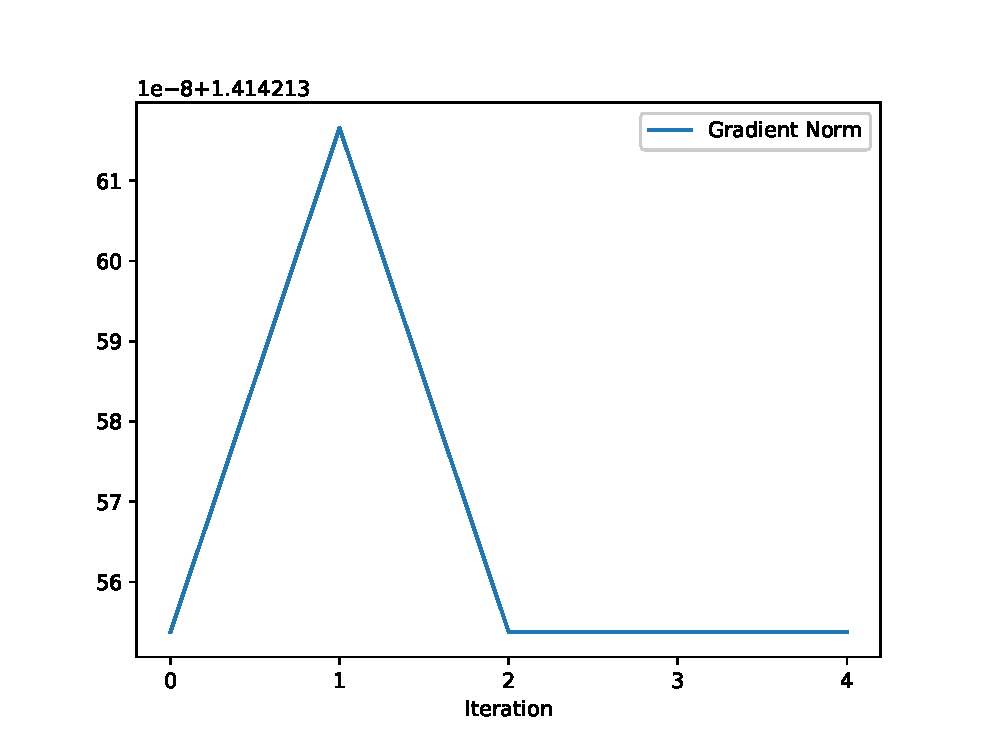
\includegraphics[width=\textwidth]{images/python/pe-pD.eps}
\caption{}
\end{subfigure}
\hfill 
\begin{subfigure}[t]{0.4\textwidth}
\centering
    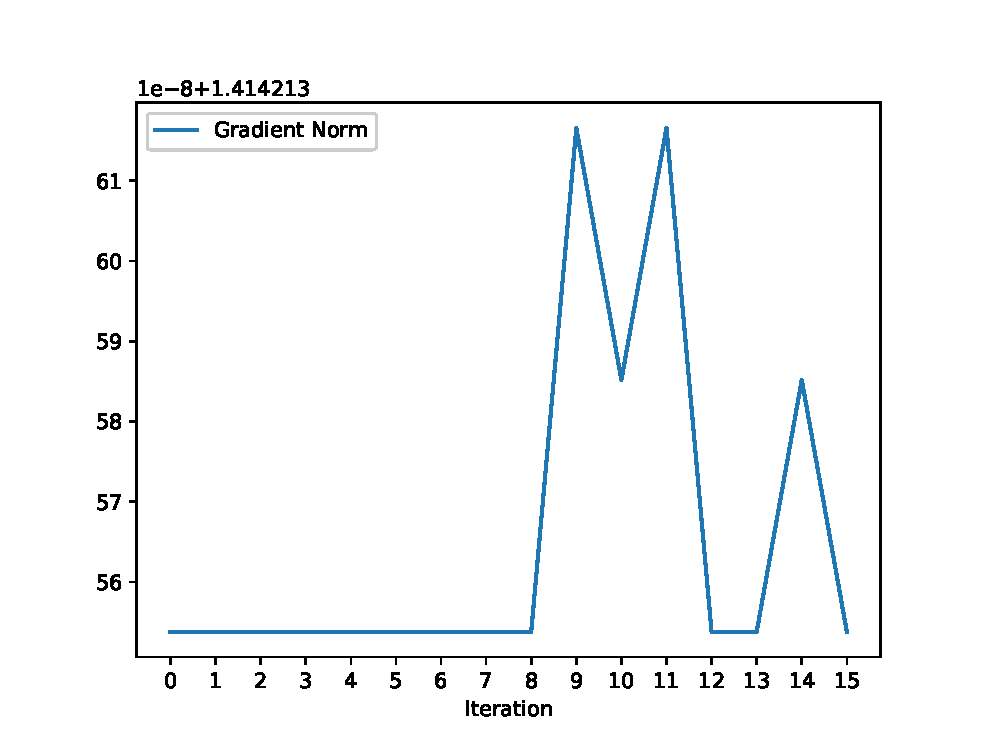
\includegraphics[width=\textwidth]{images/python/al-pD-ag.eps}
    \caption{}
\end{subfigure}
\hfill
\begin{subfigure}[t]{0.4\textwidth}
\centering
    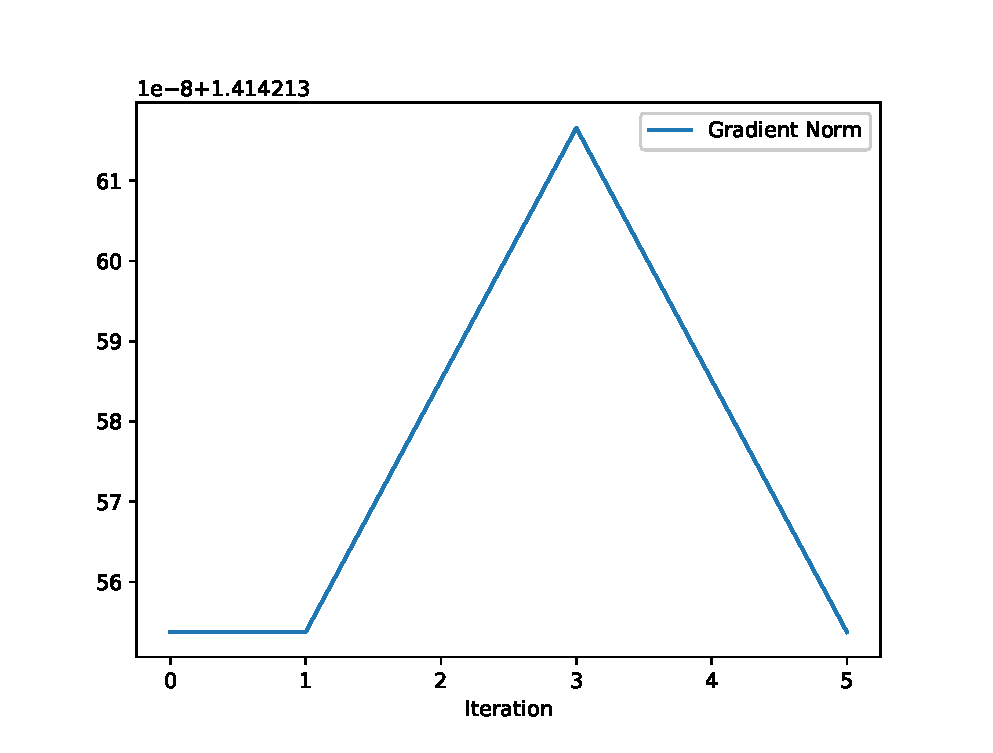
\includegraphics[width=\textwidth]{images/python/al-pD-ln.eps}
    \caption{}
\end{subfigure}
\hfill
\begin{subfigure}[t]{0.4\textwidth}
\centering
    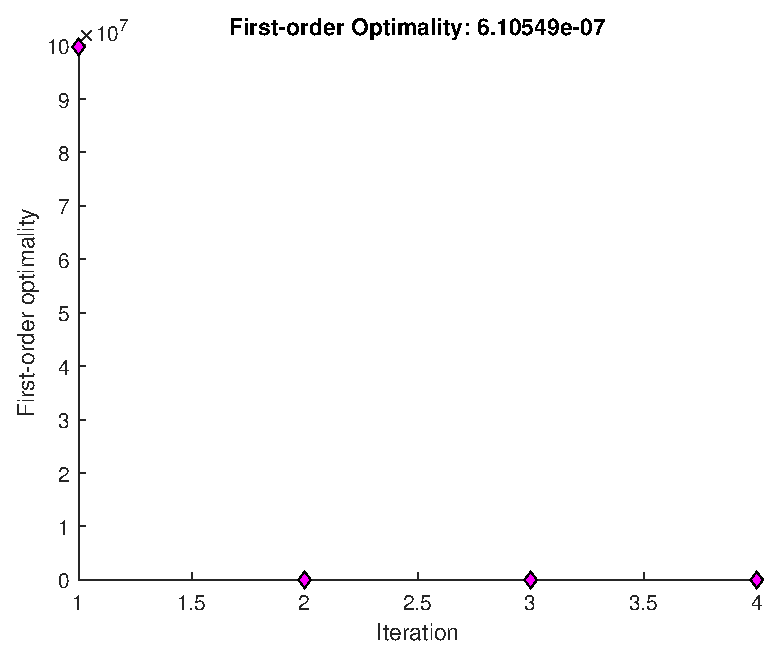
\includegraphics[width=\textwidth]{images/matlab/2a_loss.eps}
    \caption{}
\end{subfigure}
\caption{(a): Penalty, (b): Augmented Lagragrian, (c): Lagrangian, (d): Matlab: \textit{fmincon - sequential quadratic programming}}
\end{figure}
\begin{figure}
    \centering
    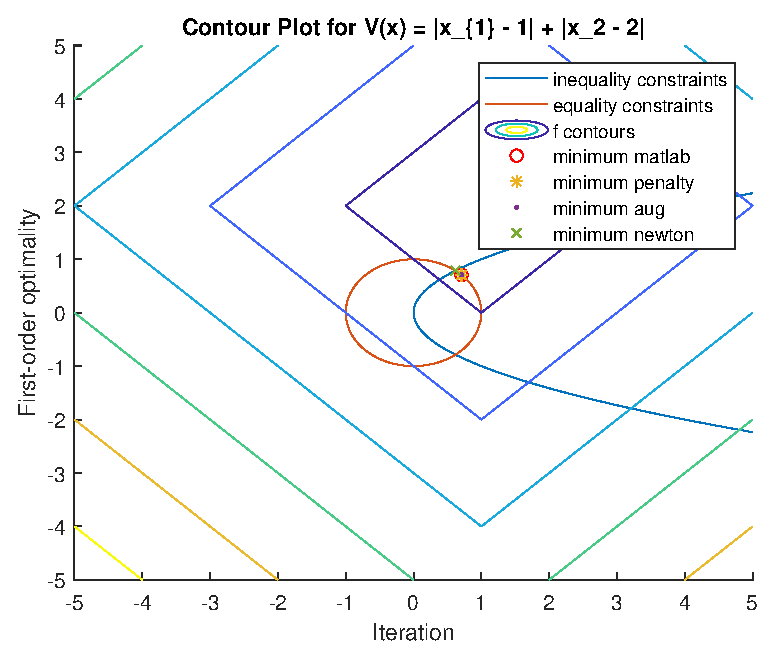
\includegraphics[width=0.4\textwidth]{images/matlab/matlab_2a.eps}
    \caption{Contour Plot for $V(x) =  | x_1 -1 | + | x_2 - 2 |$ and its constraints}
\end{figure}